\section{Image-based Rendering (渲染)}
\subsection{Rendering}
Rendering: from 3D models to images

\begin{figure}[H]
    \centering
    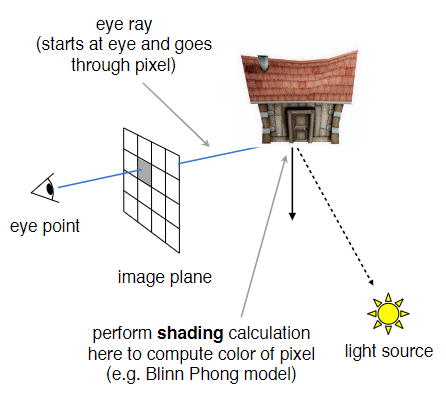
\includegraphics[width=0.418\textwidth]{Lec13/Rendering}
    \caption{Rendering}
\end{figure}

\subsection{Image-based rendering}

\begin{figure}[H]
    \centering
    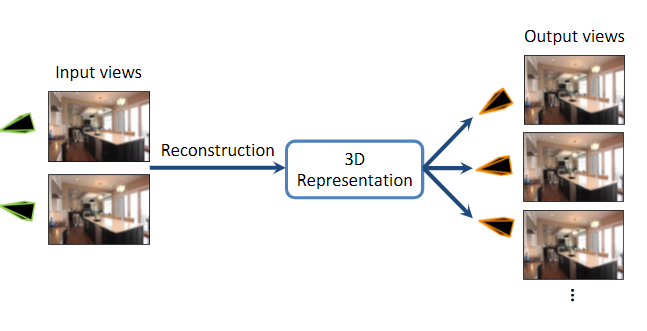
\includegraphics[width=0.618\textwidth]{Lec13/Image-based rendering}
    \caption{Image-based rendering}
\end{figure}

\subsection{Applications}
\begin{enumerate}
    \item 3D photo
    \item VR tour
    \item Bullet time effect
    \item Free-viewpoint video
    \item Immersive telepresence
    \item Embodied AI: training agents in simulated environments
\end{enumerate}

\subsection{Different representations}
\begin{enumerate}
    \item Textured mesh
    \item Light fields and Lumigraphs
    \item Depth warping
    \item Multi-plane images
    \item Neural Radiance Fields
\end{enumerate}

\subsubsection{Surface-based representations}
3D mesh with texture map

Mesh reconstruction pipeline

\begin{figure}[H]
    \centering
    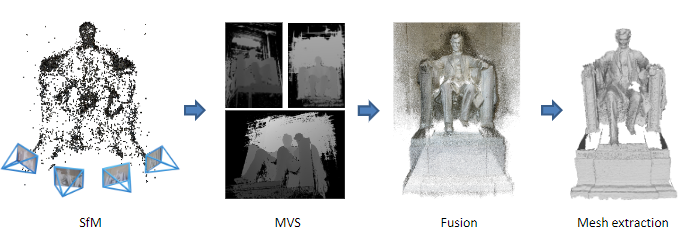
\includegraphics[width=0.618\textwidth]{Lec13/Surface-based representations}
    \caption{Surface-based representations}
\end{figure}

\textbf{Limitations:}
\begin{itemize}
    \item High-quality mesh reconstruction is difficult in many cases. 
    \item Cannot represent very complex scenes. 
\end{itemize}

\subsubsection{Light Fields}
The Plenoptic Function (7D) depicts light rays passing through:
\begin{itemize}
    \item at any location $(p_x, p_y, p_z)$. 
    \item at any viewing angle $(\theta, \phi)$. 
    \item for every wavelength $(\lambda)$. 
    \item for any time $(t)$. 
\end{itemize}
5D function by ignoring $\lambda$ and $t$. 

\begin{figure}[H]
    \centering
    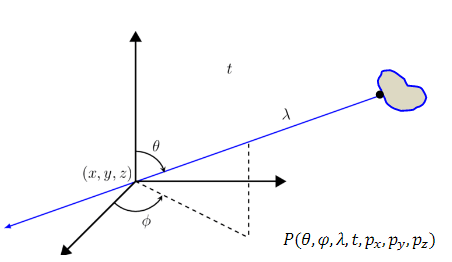
\includegraphics[width=0.418\textwidth]{Lec13/Light Fields}
    \caption{Light Fields}
\end{figure}

\textbf{Lumigraph}: approximate a light field as a 4D function (用两平面上的点确定一条光线). 

\begin{figure}[H]
    \centering
    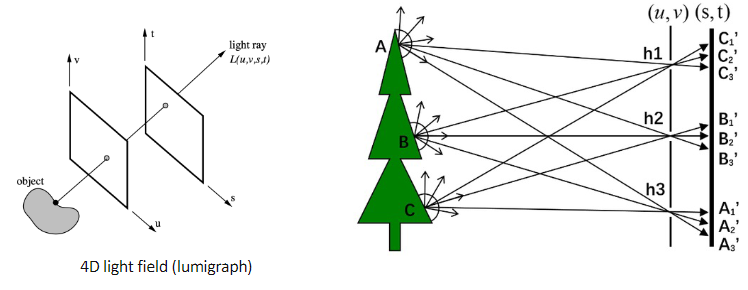
\includegraphics[width=0.618\textwidth]{Lec13/Lumigraph}
    \caption{Lumigraph}
\end{figure}

Capture the light field with a dense camera array. 

% \begin{figure}[H]
%     \centering
%     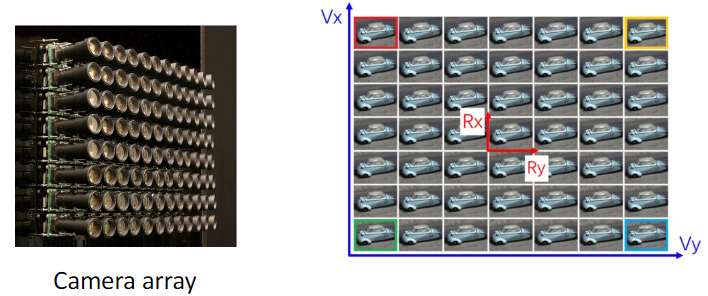
\includegraphics[width=0.618\textwidth]{Lec13/dense camera array}
%     \caption{dense camera array}
% \end{figure}

Novel view synthesis by light field interpolation. 

\begin{figure}[H]
    \centering
    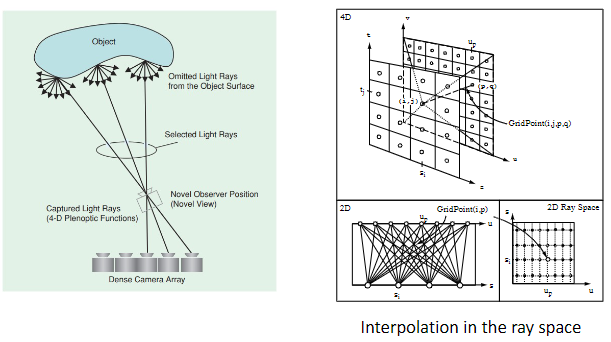
\includegraphics[width=0.518\textwidth]{Lec13/light field interpolation}
    \caption{light field interpolation}
\end{figure}

\textbf{Limitations: }
\begin{itemize}
    \item Need a dense array of cameras
    \item Can only synthesize a limited range of viewpoints
\end{itemize}

\subsubsection{Multi-Plane Image (MPI)}
A set of front-parallel planes at a fixed range of depths
Each plane encodes an RGB color image $C_d$ and an alpha/transparency map $\alpha_d$. 

\begin{figure}[H]
    \centering
    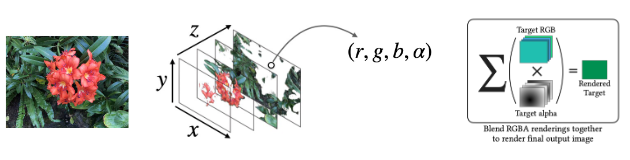
\includegraphics[width=0.618\textwidth]{Lec13/Multi-Plane Image (MPI)}
    \caption{Multi-Plane Image (MPI)}
\end{figure}

DeepView: View synthesis with learned gradient descent.

Neural Volumes: Learning Dynamic Renderable Volumes from Images. An encoder-decoder network that transforms
input images into a 3D volume representation. 

\textbf{Advantages: }
\begin{itemize}
    \item Can represent very complex scenes
    \item Realistic reflections / specularity / transparency
\end{itemize}

\textbf{Limitations: }
\begin{itemize}
    \item Discrete 3D volume requires large storage size for high-resolution rendering. 
\end{itemize}

\subsubsection{Implicit Neural Representations}
Implicit Representations is function $f_{\theta}(p)=\tau $. (使用函数表示, 需要转换才能看得到) 

\begin{figure}[H]
    \centering
    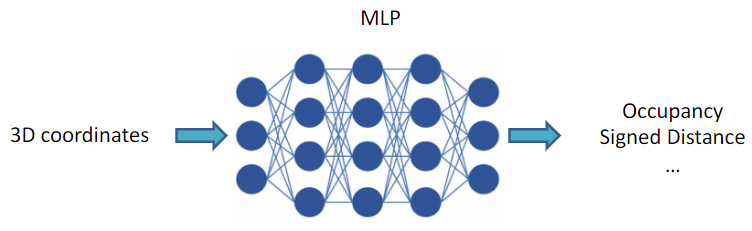
\includegraphics[width=0.618\textwidth]{Lec13/Implicit Neural Representations}
    \caption{Implicit Neural Representations}
\end{figure}

使用网络储存表达. 

\subsubsection*{Neural Radiance Fields (NeRF)}
Representing scenes as \highlight{continuous density and color fields}. 

\begin{figure}[H]
    \centering
    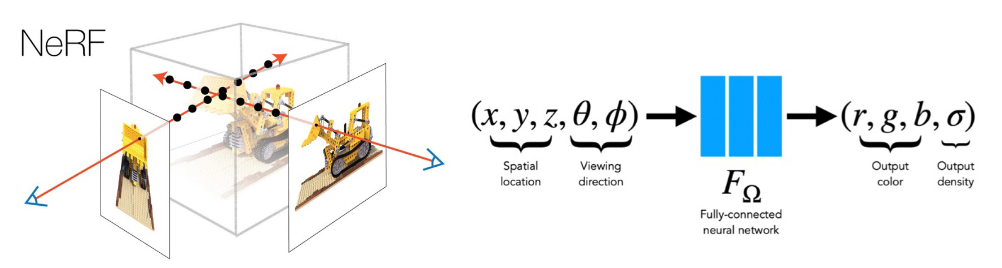
\includegraphics[width=0.618\textwidth]{Lec13/NeRF}
    \caption{NeRF}
\end{figure}

不同方向上看去的点不一样, 输入的是一个视角射线, 输出是一个点的rgb与透明度. 而且它是连续的. 

\textbf{Volume rendering}, which is differentiable. 

\begin{figure}[H]
    \centering
    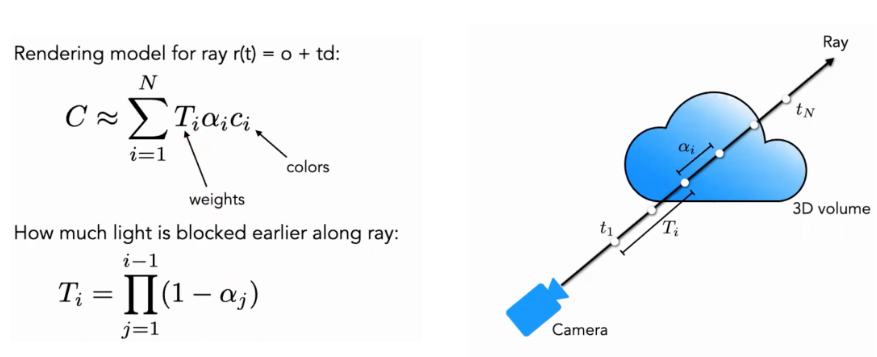
\includegraphics[width=0.618\textwidth]{Lec13/Volume rendering}
    \caption{Volume rendering}
\end{figure}

Learning NeRF from images
\begin{figure}[H]
    \centering
    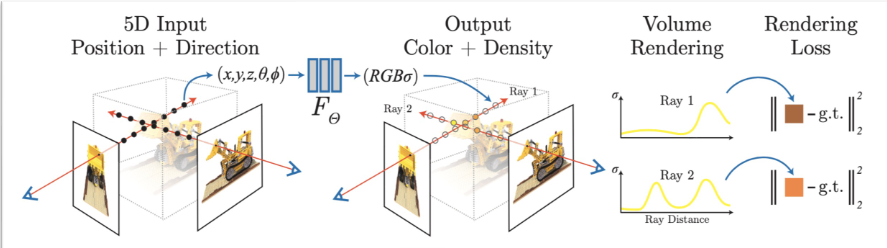
\includegraphics[width=0.618\textwidth]{Lec13/Learning NeRF from images}
    \caption{Learning NeRF from images}
\end{figure}
可微, 所以梯度下降是可用的. 

\textbf{Advantage: }
\begin{itemize}
    \item The cost to represent a 3D scene is low: 10MB. 
    \item It is a continuous and higher-resolution representation. 
    \item It can handle reflection, specularity and non-Lambertian scene well. 
\end{itemize}

\textbf{Limitation: }
\begin{itemize}
    \item Optimizing a MLP network needs about 1 day. 
    \item Render one novel view needs 30 seconds. 
    \item Only for statistic scenes and constant illumination. 
\end{itemize}

\textbf{Improvement: } 
\begin{itemize}
    \item PlenOctree for NeRF Rendering, Basic idea: 
    \begin{itemize}
        \item Offline inference: space-for-time. 
        \item Reduce memory cost by Octree. 
    \end{itemize}
    \item NeRF in the wild, Inprovement of NeRF on:
    \begin{itemize}
        \item Varying illumination of input images
        \item Removing dynamic objects in the scene. e.g. Peoples
    \end{itemize}
    \item NeuralBody: Reconstruct dynamic human body from sparse input views. 
    \item Deformable NeRF: Neural radiance field to model dynamic scenes. 
\end{itemize}
